%!TEX root = ../masters_thesis.tex

\section{Edit Hivent Data} % (fold)
\label{sec:editing_hivent_data}

The previous section proposed the abstract Hivent model, a set of Hivent operations and the HistoGraph visualization. However, one purpose of the HGIS developed in this thesis is to add, alter and delete historical changes. This section presents the tools and methods to edit spatio-temporal data about the history of Areas in the Hivent model. Whereas the Hivent operations are well-defined and specific, user studies have shown that they are not well understood by humans for edit purposes. This chapter introduces a different set of six \emph{edit operations} in section \ref{sub:edit_operations}. Afterwards, section \ref{sub:edit_workflow} shows a \emph{workflow} to perform an edit operation step by step. The Hivent model needs to support editing historical changes in between other historical changes. The last section \ref{sub:retrospective_updates} explains the theoretical approach to \emph{retrospective updates} of spatio-temporal data in the Hivent model.

% ------------------------------------------------------------------------------
\subsection{Edit Operations} % (fold)
\label{sub:edit_operations}

The Hivent operations are beneficial, because they can describe all possible changes in the development of Areas in time and space. They are well understood by the system and form the basis for the Hivent model. However, interviews with researchers in humanities at University of Virginia were conducted to understand their mental model about editing the history of countries on the map. It turned out that the Hivent operations are not suitable for a human, because of their low-level nature. One example is that the operations do not provide a simple way to create a new Area on previously unclaimed land. Changing the formal name of an Area with a \texttt{UNI} operation is also not intuitive. A main goal of this thesis is to develop a user interface that humans can understand and hence, a second set of six high-level \emph{edit operations} is proposed:

\vspace{0.5em}
\begin{table}[H]
\begin{center}
\begin{tabular}{m{0.75cm} m{0.8cm} m{2.4cm} m{9.1cm}}
  \toprule

  \raisebox{-0.35\height}
  {
\includegraphics[width=0.72cm]{graphics/development/editing_hivent_data/edit_operations/CRE}} &
  \texttt{CRE} & Create &
  \dots a new Area with a new name and territory on the map. \\

  \midrule
  \raisebox{-0.35\height}
  {
\includegraphics[width=0.72cm]{graphics/development/editing_hivent_data/edit_operations/MRG}} &
  \texttt{MRG} & Merge &
  \dots two or more Areas to a new Area. The name has to be set manually, the territory is automatically unified. \\

  \midrule
  \raisebox{-0.35\height}
  {
\includegraphics[width=0.72cm]{graphics/development/editing_hivent_data/edit_operations/SPL}} &
  \texttt{SPL} & Split &
  \dots one Area into two or more new Areas, manually setting their new territory and name. \\

  \midrule
  \raisebox{-0.35\height}
  {
\includegraphics[width=0.72cm]{graphics/development/editing_hivent_data/edit_operations/CHB}} &
  \texttt{CHB} & Change Borders &
  \dots between two neighboring Areas by defining the territory that changes sides. \\

  \midrule
  \raisebox{-0.35\height}
  {
\includegraphics[width=0.72cm]{graphics/development/editing_hivent_data/edit_operations/REN}} &
  \texttt{REN} & Rename &
  \dots an Area and set a new formal name, short name or both. \\

  \midrule
  \vspace{0.35em}
  \raisebox{-0.35\height}
  {
\includegraphics[width=0.72cm]{graphics/development/editing_hivent_data/edit_operations/DEL}} &
  \texttt{DEL} & Delete &
  \dots an Area from the map, leaving unclaimed land. \\

  \bottomrule
\end{tabular}
\caption{The six edit operations}
\label{tab:edit_operations}
\end{center}
\end{table}

% - - - - - - - - - - - - - - - - - - - - - - - - - - - - - - - - - - - - - - -
\paragraph{Error correction} % (fold)
\label{par:error_correction}

Another use case for the interface is to correct wrong information on the map. For this purpose it is important to understand how the correction of information in an event-based system works. Given an Area $A$ at $t_y$. The name of $A$ at this point should be $Y$, but happens to be $X$. That means the operation at $t_x: t_x < t_y$ that created the name $X$ for Area $A$ is erroneous and has to be corrected. Correcting a state means correcting the operation that created this state.

% paragraph error_correction (end)

% subsection edit_operations (end)

% ------------------------------------------------------------------------------
\subsection{Edit Workflow} % (fold)
\label{sub:edit_workflow}

The edit operations have proven to be understandable in several user studies. This section shows that they can be internally expressed by a set of Hivent operations. The creation of an edit operation happens in four steps:

\begin{compactenum}
  \item Select the Areas that will be changed in the operation.
  \item Create a territory for each new Area resulting from the operation.
  \item Create a name for each new Area.
  \item Add the edit operation to a Hivent to inherit the time stamp.
\end{compactenum}

For each edit operation the requirements for the steps are different. Not all operations need all steps, since some data can be processed automatically. Table \ref{tab:editoperations_in_worklow} presents an overview about the behavior of the edit operations in the first three steps. The last step is necessary for each operation.


\vspace{1em}
\begin{table}[H]
\begin{center}
\begin{tabular}{m{0.9cm} m{4.2cm} m{4.2cm} m{3.5cm}}
  \toprule

  &
  \emph{Select old Areas} &
  \emph{Create new territories} &
  \emph{Create new names} \\

  \midrule
  \raisebox{-0.35\height}
  {
\includegraphics[width=0.72cm]{graphics/development/editing_hivent_data/edit_operations/CRE}} &
  -- &
  Create a territory of the new country &
  Create a name for the new country \\

  \midrule
  \raisebox{-0.35\height}
  {
\includegraphics[width=0.72cm]{graphics/development/editing_hivent_data/edit_operations/MRG}} &
  Select the countries to be merged &
  \pbox{4.4cm}{--\\
  \emph{Territories of selected countries are automatically unified}} &
  Create a name for the new country
  \\

  \midrule
  \raisebox{-0.35\height}
  {
\includegraphics[width=0.72cm]{graphics/development/editing_hivent_data/edit_operations/SPL}} &
  Select a country to be \mbox{split} &
  Create a territory for each new country &
  Create a name for each new country \\

  \midrule
  \raisebox{-0.35\height}
  {
\includegraphics[width=0.72cm]{graphics/development/editing_hivent_data/edit_operations/CHB}} &
  Select two neighboring countries to change their border &
  \pbox{4.4cm}{Create a new border between both countries \\
  \emph{The territories of both countries are created automatically}}  &
  -- \\

  \midrule
  \raisebox{-0.35\height}
  {
\includegraphics[width=0.72cm]{graphics/development/editing_hivent_data/edit_operations/REN}} &
  Select a country to rename it &
  -- &
  Create a new name of the country \\

  \midrule
  \raisebox{-0.35\height}
  {
\includegraphics[width=0.72cm]{graphics/development/editing_hivent_data/edit_operations/DEL}} &
  Select a country to delete it &
  -- &
  -- \\

  \bottomrule
\end{tabular}
\caption{The requirements of each step for the edit operations}
\label{tab:editoperations_in_worklow}
\end{center}
\end{table}

% - - - - - - - - - - - - - - - - - - - - - - - - - - - - - - - - - - - - - - -

% wording:
% UNI of "[old]"  to    "new"
% INC of "[old]"  into  "pres"
% SEP of "old"    into  "[new]"
% SEC of "[new]"  from  "pres"
% NCH of "pres"

\vspace{-1.0em}

There are different possibilities to express an edit operation by a set of Hivent operations, depending on the user input in the workflow. All possibilities are introduced in table \ref{tab:editoperations_to_hg_operations}. Hivent operations are combined when they happen at the same time. In the example of the German Reunification, East Germany was incorporated into West Germany which at the same time changed its short name to ``Germany'' (\texttt{INC + NCH}).

\begin{center}
\begin{longtable}{m{1.2cm} m{0.95cm} m{0.95cm} m{0.95cm} m{6.0cm} m{2.3cm}}
  \toprule

  \pbox{1.2cm}{Edit \\ operation\\[-1.2em]} &
  \pbox{0.95cm}{Old\\Areas\\[-1.2em]} &
  \pbox{0.95cm}{Update\\Areas\\[-1.2em]} &
  \pbox{0.95cm}{New\\Areas\\[-1.4em]} &
  Expression by Hivent operations \protect\footnotemark &
  Visualization \\
  \midrule
  \endhead

  %%% CREATE %%

  \multirow{9}{*}{\texttt{CRE} (1)} &
  \multicolumn{4}{p{10cm}}{
    Area $B_1$ is created with territory $T$. The part of $T$ that is on previously unclaimed land ($T_\Omega$) is seceded as $B_1$ from $\Omega$.
    If $T_\Omega$ is empty, then $B_1$ is initialized with an empty territory.
    The rest of $T$ covers some Areas $P_i \in P$ partially and some Areas $F_i \in F$ fully.
    $\forall P_i:$ The covered territory $T_i$ is seceded and incorporated into $B_1$.
    $\forall F_i: F_i$ is completely incorporated into $B_1$.
  } &
  \multirow{9}{*}{
    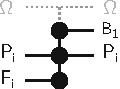
\includegraphics[width=2.5cm]{graphics/development/editing_hivent_data/edit_to_hivent_operations/CRE_to_SEC+UNI}
  } \\
  & \\[-0.85em]
  &
  $\forall F_i$ &
  $\forall P_i$ &
  $B_1$ &
  \pbox{6.0cm}{
    \texttt{SEC} of $B_1$ from $\Omega$ \\
    \texttt{SEC} of $T_i$ from $P_i$, \texttt{INC} of $T_i$ into $B_1$ \\
    \texttt{INC} of $F_i$ into $B_1$
  } &
  \\

  %%% MERGE %%

  \midrule
  \multirow{4}{*}{\texttt{MRG} (1)} &
  \multicolumn{4}{p{10cm}}{
    Multiple Areas $A_i \in A, |A| \geq 2$ are unified to $B_1$. The new Area receives a name distinct from all names of $A_i$.
  } &
  \multirow{4}{*}{
    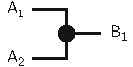
\includegraphics[width=2.5cm]{graphics/development/editing_hivent_data/edit_to_hivent_operations/MRG_to_UNI}
  } \\
  & \\[-0.85em]
  &
  $\forall A_i$ &
  -- &
  $B_1$ &
  \pbox{6.0cm}{
    \texttt{UNI} of $\forall A_i$ to $B_1$
  } &
  \\

  \midrule
  \multirow{4}{*}{\texttt{MRG} (2)} &
  \multicolumn{4}{p{10cm}}{
    Multiple Areas $A_i \in A, |A| \geq 2$ are unified. The resulting Area reuses the short and formal name of one of the old Areas ($A_0$) and therefore preserves it. The remaining Areas $A_i$ are incorporated into $A_0$.
  } &
  \multirow{4}{*}{
    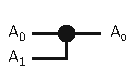
\includegraphics[width=2.5cm]{graphics/development/editing_hivent_data/edit_to_hivent_operations/MRG_to_INC}
  } \\
  & \\[-0.85em]
  &
  $\forall A_i$ &
  $A_0$ &
  -- &
  \pbox{6.0cm}{
    \texttt{INC} of $\forall A_i$ into $A_0$
  } &
  \\

  \midrule
  \multirow{4}{*}{\texttt{MRG} (3)} &
  \multicolumn{4}{p{10cm}}{
    The same as the previous case, but $A_0$ receives a new short name and therefore an additional name change is required.
  } &
  \multirow{4}{*}{
    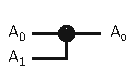
\includegraphics[width=2.5cm]{graphics/development/editing_hivent_data/edit_to_hivent_operations/MRG_to_INC+NCH}
  } \\
  & \\[-0.85em]
  &
  $\forall A_i$ &
  $A_o$ &
  -- &
  \pbox{6.0cm}{
    \texttt{INC} of $\forall A_i$ into $A_0$ \\
    \texttt{NCH} of $A_0$
  } &
  \\

  %%% SPLIT %%

  \midrule
  \multirow{4}{*}{\texttt{SPL} (1)} &
  \multicolumn{4}{p{10cm}}{
    Multiple Areas $B_i$ are separated from one initial Area $A_1$. Each $B_i$ receives a part of the territory of $A_1$ and a name. Each name is distinct from the name of $A_1$.
  } &
  \multirow{4}{*}{
    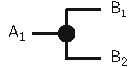
\includegraphics[width=2.5cm]{graphics/development/editing_hivent_data/edit_to_hivent_operations/SPL_to_SEP}
  } \\
  & \\[-0.85em]
  &
  $A_1$ &
  -- &
  $\forall B_i$ &
  \pbox{6.0cm}{
    \texttt{SEP} of $A_1$ into $\forall B_i$
  } &
  \\

  \midrule
  \multirow{5}{*}{\texttt{SPL} (2)} &
  \multicolumn{4}{p{10cm}}{
    Multiple Areas $B_i$ are separated from one initial Area $A_0$. Each $B_i$ receives a part of the territory of $A_0$ and a name. One of the separated Areas has the same short and formal name as $A_0$, so it preserves its identity. The remaining new Areas secede from $A_0$.
  } &
  \multirow{5}{*}{
    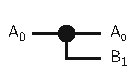
\includegraphics[width=2.5cm]{graphics/development/editing_hivent_data/edit_to_hivent_operations/SPL_to_SEC}
  } \\
  & \\[-0.85em]
  &
  -- &
  $A_0$ &
  $\forall B_i$ &
  \pbox{6.0cm}{
    \texttt{SEC} of $\forall B_i$ from $A_0$
  } &
  \\

  \midrule
  \pagebreak
  \multirow{3}{*}{\texttt{SPL} (3)} &
  \multicolumn{4}{p{10cm}}{
    The same as the previous case, but $A_0$ receives a new short name and therefore an additional name change is required.
  } &
  \multirow{3}{*}{
    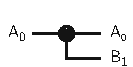
\includegraphics[width=2.5cm]{graphics/development/editing_hivent_data/edit_to_hivent_operations/SPL_to_SEC+NCH}
  } \\
  & \\[-0.85em]
  &
  -- &
  $A_0$ &
  $\forall B_i$ &
  \pbox{6.0cm}{
    \texttt{SEC} of $\forall B_i$ from $A_0$  \\
    \texttt{NCH} of $A_0$
  } &
  \\

  %%% CHANGE BORDER %%%

  \midrule
  \multirow{10}{*}{\texttt{CHB} (1)} &
  \multicolumn{4}{p{10cm}}{
    One existing Area $A_0$ is selected and its territory changes.
    Relative to the old territory,
    some parts of the territory expands ($T_e$) and some withdraw ($T_w$).
    The part of $T_e$ that expands into unclaimed land ($T_\Omega: T_\Omega \in T_e$) is seceded from $\Omega$ and incorporated into $A_0$.
    The Areas $F_i$ which are fully covered by $T_e$ are incorporated into $A_0$,
    the Areas $P_i$ partially covered by $T_e$ secede this territory $T_i \in T_e$ to $A_0$.
    $T_w$ is incorporated into $\Omega$, resulting in unclaimed land.
  } &
  \multirow{10}{*}{
    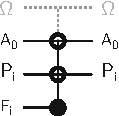
\includegraphics[width=2.5cm]{graphics/development/editing_hivent_data/edit_to_hivent_operations/CHB_to_SEC+INC_omega}
  } \\
  & \\[-0.85em]
  &
  $\forall F_i$ &
  $A_0, \forall P_i$ &
  -- &
  \pbox{6.0cm}{
    \texttt{SEC} of $T_\Omega$ from $\Omega$,
                                        \texttt{INC} of $T_\Omega$ into $A_0$ \\
    \texttt{SEC} of $T_i$ from $P_i$,   \texttt{INC} of $T_i$ into $A_0$ \\
    \texttt{INC} of $F_i$ into $A_0$ \\
    \texttt{SEC} of $T_w$ from $A_0$,   \texttt{INC} of $T_w$ into $\Omega$
  } &
  \\

  \midrule
  \multirow{7}{*}{\texttt{CHB} (2)} &
  \multicolumn{4}{p{10cm}}{
    Two existing Areas $A_1$ and $A_2$ are selected and their common border changes.
    This results in a symmetrical change of territories, made up by two sets of territories:
    $T_2$, that previously belonged to $A_1$ and is now part of $A_2$, and $T_1$ for which the opposite is true.
    $T_2$ is seceded by $A_1$ and incorporated into $A_2$, the opposite happens to $T_1$.
  } &
  \multirow{7}{*}{
    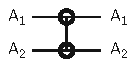
\includegraphics[width=2.5cm]{graphics/development/editing_hivent_data/edit_to_hivent_operations/CHB_to_SEC+INC}
  } \\
  & \\[-0.85em]
  &
  -- &
  $A_1, A_2$ &
  -- &
  \pbox{6.0cm}{
    \texttt{SEC} of $T_2$ from $A_1$,
    \texttt{INC} of $T_2$ into $A_2$ \\
    \texttt{SEC} of $T_1$ from $A_2$,
    \texttt{INC} of $T_1$ into $A_1$
  } &
  \\

  %%% RENAME %%%

  \midrule
  \multirow{4}{*}{\texttt{REN} (1)} &
  \multicolumn{4}{p{10cm}}{
    One Area $A_1$ is selected and both its short and formal name is changed. Therefore, a new Area $B_1$ is created as a direct successor of $A_1$. This is a special case of a unification with only one Area.
  } &
  \multirow{4}{*}{
    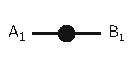
\includegraphics[width=2.5cm]{graphics/development/editing_hivent_data/edit_to_hivent_operations/REN_to_UNI}
  } \\
  & \\[-0.85em]
  &
  $A_1$ &
  -- &
  $B_1$ &
  \pbox{6.0cm}{
    \texttt{UNI} of $A_1$ to $B_1$
  } &
  \\

  \midrule
  \multirow{3}{*}{\texttt{REN} (2)} &
  \multicolumn{4}{p{10cm}}{
    One Area $A_1$ is selected and receives a new short name, but the formal name and therefore the identity is preserved. $A_1$ is updated.
  } &
  \multirow{3}{*}{
    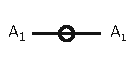
\includegraphics[width=2.5cm]{graphics/development/editing_hivent_data/edit_to_hivent_operations/REN_to_NCH}
  } \\
  & \\[-0.85em]
  &
  -- &
  $A_1$ &
  -- &
  \pbox{6.0cm}{
    \texttt{NCH} of $A_1$
  } &
  \\

  %%% CEASE %%%

  \midrule
  \multirow{2}{*}{\texttt{DEL} (1)} &
  \multicolumn{4}{p{10cm}}{
    One Area $A_1$ is selected and deleted by incorporating into the universe.
  } &
  \multirow{2}{*}{
    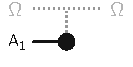
\includegraphics[width=2.5cm]{graphics/development/editing_hivent_data/edit_to_hivent_operations/DEL_to_INC}
  } \\
  & \\[-0.85em]
  &
  $A_1$ &
  -- &
  -- &
  \pbox{6.0cm}{
    \texttt{INC} of $A_1$ into $\Omega$
  } &
  \\

  \bottomrule
\caption{Translation from edit operations to Hivent operations}
\label{tab:editoperations_to_hg_operations}
\end{longtable}
\footnotetext{
  Multiple Hivent operations in one row happen exactly at the same moment and thus are combined.
}
\end{center}


% subsection edit_workflow (end)

% ------------------------------------------------------------------------------
\subsection{Retrospective Updates} % (fold)
\label{sub:retrospective_updates}

A straightforward use case of the Hivent model is to change the current state of the system with a new Hivent operation into the future. Given are the initial start point $t_0$, a current point $t_{now} > t_0$ and a set of consecutively added Hivent operations at $\forall t_i: t_0 \leq t_i < t_{now}$. The accumulation of all changes make up the current state of the system at $t_{now}$. In order to change this current state, a new Hivent operation can be inserted at $t_{now}$ into the future. This state is valid until the next change is inserted. For historical research this use case alone is not sufficient, because the current state of the map at $t_{now}$ is known to a large degree. The problem is to describe changes in the past. Therefore, the system needs to support retrospective insertion of Hivent operations in between existing operations and therefore update the set of Hivent operations in the system.
Each Hivent operation that is not added to the end of the timeline must maintain the semantic, spatial and thematic integrity of the data, i.e.\ the changes to Areas, their territories and names must still work.

\begin{figure}[H]
  \vspace{1em}
  \centering
  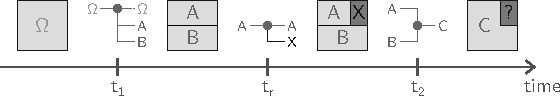
\includegraphics[width=0.73\textwidth]{graphics/development/editing_hivent_data/retrospective_updates/example}
  \caption{Example for a simple conflict due to a retrospective update}
  \label{fig:update_conflict_example}
\end{figure}

The example in figure \ref{fig:update_conflict_example} illustrates the problem: Given $t_1$ with two Areas $A$ and $B$ and a \texttt{UNI} operation at $t_2$ unifying $A$ and $B$ to $C$. A \texttt{SEC} of a new Area $X$ from $A$ is inserted at $t_r: t_1 < t_r < t_2$ in retrospective. The operation at $t_2$ is not consistent any more, because the old territory of $A$ is not the same. It is not simple to say how the remaining territory `$?$' should be treated.


% - - - - - - - - - - - - - - - - - - - - - - - - - - - - - - - - - - - - - - -
\paragraph{Conflicts} % (fold)
\label{par:conflicts}

The way the Hivent model works is comparable to a version control system like \emph{Git}. There are different kinds of conflicts that can occur on retrospective updates. In the Hivent model, they are classified regarding their resolvability:

\begin{compactitem}
  \item[A)] The conflict can be resolved \emph{\textbf{a}utomatically} without the interference of the user.
  \item[S)] The conflict requires the user to choose between two alternatives (\emph{\textbf{s}emi-automatic} resolution).
  \item[M)] The conflict is complex and the user needs to resolve it \emph{\textbf{m}anually}.
\end{compactitem}

The remaining part of this section examines all possible cases of conflicts and their resolvability. Each inserted Hivent operation transforms a set of old Areas $A = [A_i]$ to a set of new Areas $B = [B_i]$ or updates an update Area $A_0$ or does both. Each consecutive Hivent operation that manipulates $A_0, A_i \in A$ or $B_i \in B$ has to be checked regarding three aspects of integrity:

\begin{compactenum}
  \item semantic: Does $A_0$ and $\forall A_i \in A$ still exist? If not, can it easily be replaced by another Area?
  \item spatial: Is the territory of $A_0$ and $\forall A_i \in A$ still the same? If not, can it easily be updated?
  \item thematic: Is the name of $A_0$ and $\forall A_i \in A$ still the same? If not, can it easily be updated?
\end{compactenum}

All cases can be simulated in the following simple scenario:
The system has only two states, an initial state at $t_1$ at which only three spatial entities are on the map ($A_1, A_2, A_3$) and a Hivent operation at $t_2$ that manipulates some of these Areas with one of the five possible operations. This is called the original Hivent operation ($H_o$). Now a retrospective update $H_r$ is inserted in between the two states ($t_r: t_1 < t_r < t_2$). $H_r$ manipulates the same set of Areas with a Hivent operation. The question is: What happens to the semantic, spatial and thematic integrity of $H_o$? Is there a conflict and if so, how can it be resolved? There are 25 possible cases, because there are five possible Hivent operations for both $H_o$ and $H_r$.

% paragraph conflicts (end)

% - - - - - - - - - - - - - - - - - - - - - - - - - - - - - - - - - - - - - - -
\paragraph{Retrospective Name Change} % (fold)
\label{par:retrospective_name_change}

The first five cases are straightforward: Assuming \texttt{NCH} is inserted in retrospective ($H_r$) to change the name of $A_1$ from $X$ to $Y$. This has no effect on the identity or territory of $A_1$. Therefore, the system only needs to check for thematic integrity of $H_o$. If that operation is an \texttt{INC} or \texttt{SEC}, which both only change the territory of $A_1$, it is not conflicting. If $H_o$ is a \texttt{UNI} or \texttt{SEP}, then there is a conflict: $A_1$ is an old Area of the operation, but the name associated to $A_1$ is still $X$. This is not consistent, because $H_r$ just changed the name to $Y$. This conflict can be resolved automatically by updating the name in the old Area from $X$ to $Y$. The same is true if $H_o$ is a \texttt{NCH} operation: $A_1$ is the update Area and the old name has to be updated from $X$ to $Y$. To summarize what the system has to do if a \texttt{NCH} on $A_1$ is inserted in retrospective: find the next \texttt{UNI}, \texttt{SEP} or \texttt{NCH} operation that manipulates $A_1$ and update its old name.

% paragraph retrospective_name_change (end)

% - - - - - - - - - - - - - - - - - - - - - - - - - - - - - - - - - - - - - - -
\paragraph{Retrospective Incorporation} % (fold)
\label{par:retrospective_incorporation}

An \texttt{INC} deletes a set of old Areas and changes the territory of one Area. In this scenario, $H_r$ incorporates $A_2$ into $A_1$. The question is what kind of conflicts can occur to the spatial integrity of $H_o$? If $H_o$ is  a \texttt{NCH}, there is no conflict, because $H_o$ changes the territory of $A_1$ and \texttt{NCH} the name. However, there might be a conflict in the next operation that manipulates $A_1$.

\begin{figure}[ht]
\vspace{1em}
  \centering
  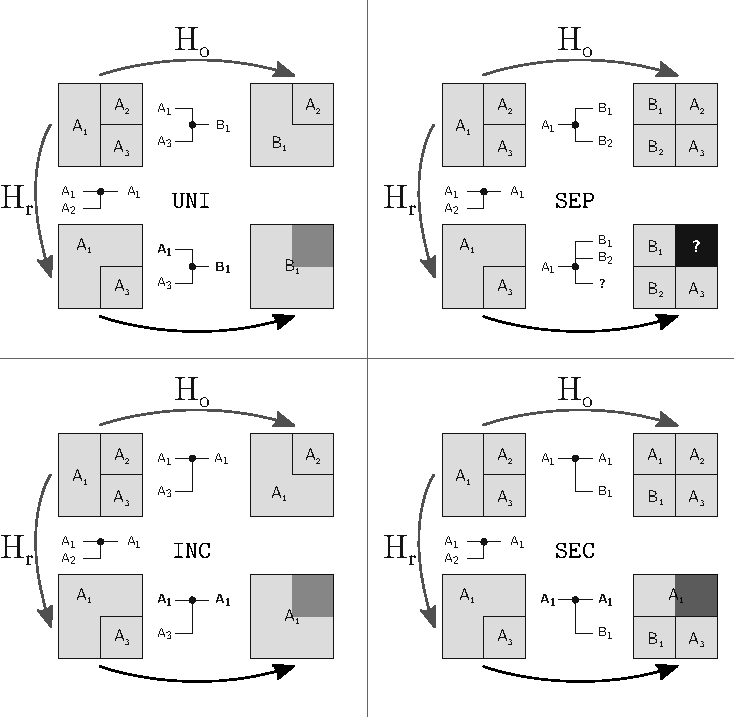
\includegraphics[width=0.9\textwidth]{graphics/development/editing_hivent_data/retrospective_updates/INC}
  \caption{Conflicts after a retrospective incorporation}
  \label{fig:update_conflict_INC}
\end{figure}

Figure \ref{fig:update_conflict_INC} illustrates the conflicts that occur in the remaining possibilities for $H_o$. In case of an original \texttt{UNI} operation, it can still be performed with the same Areas, because $H_r$ did not change the identity of $A_1$. However, the territory of $A_1$ has been enlarged. This new territory influences $H_o$. In order to maintain spatial integrity, the system has to update the territory of incoming $A_1$. The territory of $B_1$ has to be updated as well, because it is enlarged in the same way as $A_1$. This requires a \emph{recursive update} into the future: the next Hivent operation dealing with $B_1$ needs to take into account that the territory has changed. This case can be treated as if $H_o$ would be $H_r$ with an \texttt{INC} operation. This update can cause new conflicts that either the system or the user have to solve, which can then lead to new conflicts again, etc. The system has to repeat this process into the future until all conflicts are resolved. The same is true if $H_o$ is an \texttt{INC} operation: the system needs to update the old and new territory of $A_1$ in $H_o$ and recursively update the territory of $A_1$ into the future.

If $H_o$ is a \texttt{SEP} operation, there is a major conflict: Originally, $A_1$ split into $B_1$ and $B_2$. The territory of $A_1$ is larger due to $H_r$. $H_o$ can still separate $B_1$ and $B_2$ from $A_1$ the same way as before, but it is uncertain what should happen to the remaining territory of $A_1$ that has just been enlarged. This conflict has to be resolved manually, because the system cannot derive a decision from any existing information. The remaining part could either become $\Omega$, or it could be incorporated into $B_1$ or $B_2$, or stay $A_1$. However, the user has to decide. In case of an original \texttt{SEC}, the situation is slightly different: $H_1$ still exists as before, just with a larger territory. $H_o$ can secede $B_1$ as in the first place, but the system needs to update the old and new territory of $A_1$ in this operation and recursively into the future.

The foregoing investigation relates only to $A_1$, but not to $A_2$ that has been incorporated into $H_r$. From the perspective of $A_2$, this change can be seen as a \texttt{UNI}, because its identity is deleted and together with its territory it completely merges into $A_1$. Therefore, this is treated like a retrospective unification examined later in this section.

% paragraph retrospective_incorporation (end)

% - - - - - - - - - - - - - - - - - - - - - - - - - - - - - - - - - - - - - - -
\paragraph{Retrospective Secession} % (fold)
\label{par:retrospective_secession}

Retrospective secessions are comparable to incorporations. The identity and the name of $A_1$ does not change -- but parts of its territory secedes to a new Area $B_1$. This section examines how the system has to treat $B_1$ and the smaller territory of $A_1$ in the original operation $H_o$. Exactly as for retrospective incorporation, there is no conflict if $H_o$ is a \texttt{NCH}, but possibly later.

\begin{figure}[ht]
\vspace{1em}
  \centering
  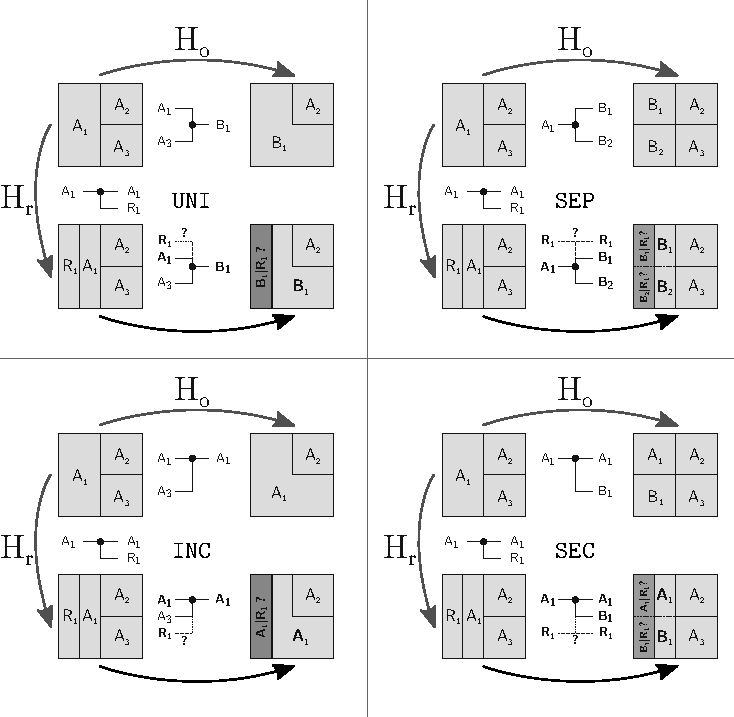
\includegraphics[width=0.9\textwidth]{graphics/development/editing_hivent_data/retrospective_updates/SEC}
  \caption{Conflicts after a retrospective secession}
  \label{fig:update_conflict_SEC}
\end{figure}

The other four cases are visualized in figure \ref{fig:update_conflict_SEC}. For an original \texttt{UNI}, there is a conflict: Originally, $A_1$ and $A_3$ unified to $B_1$. Although $H_r$ cedes parts of the territory of $A_1$ to $R_1$, $H_o$ can still merge it with $A_3$. The question is what happens to the remaining territory of $R_1$? There are two options:
\begin{compactenum}
  \item
  \emph{priority to $H_r$}:
  $R_1$ stays an own Area and is not affected by $H_o$.
  \item
  \emph{priority to $H_o$}:
  $H_o$ unifies $R_1$ to $B_1$ as well.
\end{compactenum}

For the system it is hard to make a decision, because the user's intention when creating $R_1$ in $H_r$ is not clear: should the newly created Area remain there or is the territory of the united Area $A_3$ more important? In order for the system to not behave unexpectedly, it will ask the user which choice they prefer. In case of the first choice, the territory of $R_1$ has to be subtracted from the territory of the new Area $B_1$ in $H_o$. This update is again recursive, because the next Hivent operation dealing with $B_1$ needs to operate on the correct territory as well. In the second case, $R_1$ simply has to be added to the old Areas of the \texttt{UNI} operation in $H_o$. No further recursive update is necessary. The same behavior is true if $H_o$ is an \texttt{INC}. The user has to decide if they want to incorporate $R_1$ into $A_1$ or keep it as a separate Area. In the latter case, the system needs to update the new territory of $A_1$ in $H_o$.

For an original \texttt{SEP}, the situation is comparable: Originally, $A_1$ splits into $B_1$ and $B_2$, but after the retrospective secession of a part of $A_1$ to $R_1$, the territory of $R_1$ conflicts with $B_1$ and $B_2$ in $H_o$. An important observation is that each part of $R_1$ would be part of either $B_1$ or $B_2$. There is no remaining land, since both $R_1$ and $B_1+B_2$ seceded from the same territory of $A_1$. Just like the other two cases above, the system will give the user the choice for both conflicting territories if either $R_1$ should stay an Area or if $B_1$ or $B_2$ should incorporate $R_1$ into their territory. In the first case, the territory of $R_1$ has to be subtracted from both the incoming $A_1$ and recursively from the outgoing territory $B_1$ or $B_2$. The latter case needs at least one additional Hivent operation: The part of $R_1$ that shall be part of $B_1$ or $B_2$ needs to be seceded from $R_1$, and in the same moment incorporated into $A_1$. $A_1$ itself is separated into $B_1$ and $B_2$ at the same time: $H_o$ = \texttt{SEC+INC+SEP}. If $R_1$ is entirely deleted in the operation, then it is completely incorporated into $A_1$, so it is only an \texttt{INC+SEP} at $H_o$. The case of an original \texttt{SEC} the system behaves in exactly the same way, just with an update of the territory of $A_1$ and $B_1$ instead of $B_1$ and $B_2$.

To summarize, the main difference between retrospective incorporation and secession is that in the latter case, the user needs to choose between two predefined options. For incorporations, this is seen as unnecessary, because the conflicting territory of $A_2$ has not been manipulated by $H_o$ and hence, it cannot be seen as a conscious decision of the user to keep this Area.

% paragraph retrospective_secession (end)

% - - - - - - - - - - - - - - - - - - - - - - - - - - - - - - - - - - - - - - -
\paragraph{Retrospective Unification} % (fold)
\label{par:retrospective_unification}

If a \texttt{UNI} is inserted in retrospective, the semantic integrity of $H_o$ is threatened, because in contrast to a \texttt{INC} all incoming Areas unify to one completely new Area, in this example $R_1$. For each Area $A_i \in A$ that was unified in $H_r$ the system needs to find the next Hivent operation $H_o$ that manipulates $A_i$ and update it accordingly. In this example, $A_1$ is examined in place of each $A_i \in A$. If $H_o$ is a \texttt{NCH}, there is a conflict: the name of $A_1$ can obviously not be updated any more, because $A$ is already deleted. The only way to resolve this conflict is to automatically delete the \texttt{NCH} operation. The remaining four cases behave in exactly the same way regarding spatial integrity as for a retrospective incorporation -- with the only difference that the Area $A_1$ is replaced by $R_1$ as an incoming Area in the operation. In all four cases, the territory has to be updated in the same way as for retrospective incorporation and the same conflict occurs for the original \texttt{SEP} operation.

\begin{figure}[ht]
\vspace{1em}
  \centering
  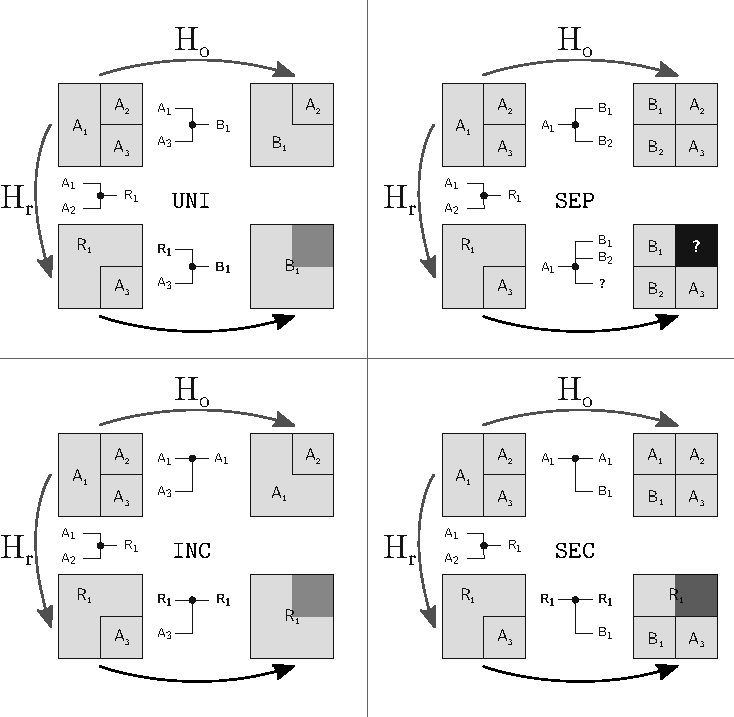
\includegraphics[width=0.9\textwidth]{graphics/development/editing_hivent_data/retrospective_updates/UNI}
  \caption{Conflicts after a retrospective unification}
  \label{fig:update_conflict_UNI}
\end{figure}

% paragraph retrospective_unification (end)

% - - - - - - - - - - - - - - - - - - - - - - - - - - - - - - - - - - - - - - -
\paragraph{Retrospective Separation} % (fold)
\label{par:retrospective_separation}

In contrast to the previous example, retrospective separations behave slightly different from secessions. $H_o$ has to be checked both for spatial and semantic integrity, since $A_1$ is deleted in $H_r$ to a set of new Areas $R_i$. In this scenario, $R_1$ and $R_2$ stay in place for $\forall r_i \in R$. If $H_o$ is a \texttt{NCH}, the operation has to be automatically deleted, because $A_1$ does not exist any more. Figure \ref{fig:update_conflict_SEP} shows the conflicts that arise for the remaining four cases.

\begin{figure}[ht]
\vspace{1em}
  \centering
  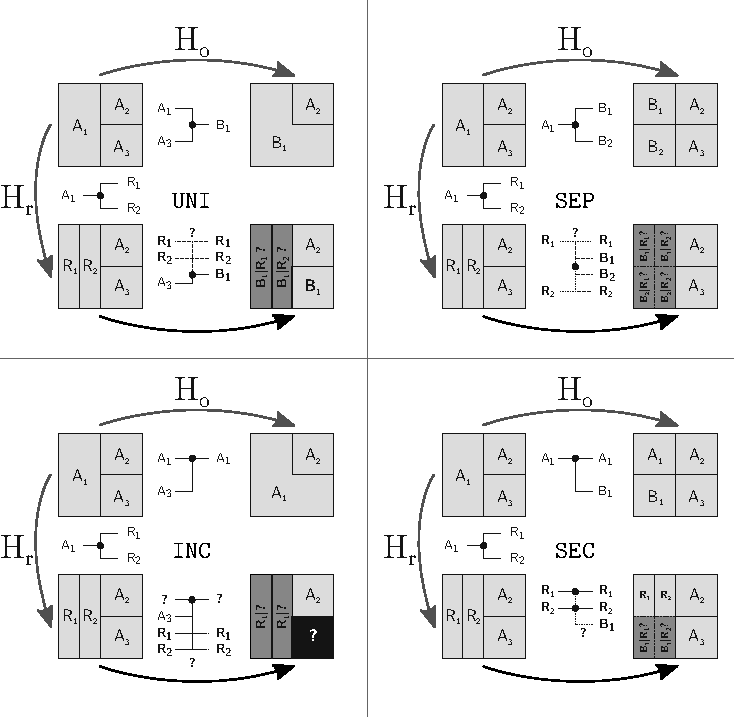
\includegraphics[width=0.9\textwidth]{graphics/development/editing_hivent_data/retrospective_updates/SEP}
  \caption{Conflicts after a retrospective separation}
  \label{fig:update_conflict_SEP}
\end{figure}

In case $H_o$ is a \texttt{UNI}, the arising conflict can be solved semi-automatically. Originally, $B_1$ was created by unifying $A_1$ and $A_3$. $A_1$ just got separated into $R_1$ and $R_2$ by $H_r$, so the system cannot know if $R_1$, $R_2$ or $B_1$ is preferred at $H_o$. In any case, the system needs to remove $A_1$ from the old Areas in the \texttt{UNI} operation. For each Area created in $H_r$ -- in this case only $R_1$ and $R_2$ -- the system asks the user if they prefer $R_i$ or $B_1$. If $R_1$ is preferred, then its territory has to be recursively subtracted from the outgoing Area $B_1$ in the \texttt{UNI} operation at $H_o$. Otherwise, $R_i$ is added to the old Areas of $H_o$. If $R_i$ is preferred every time, the remaining \texttt{UNI} operation only transforms $A_3$ to $B_1$.

If $H_o$ is an \texttt{INC}, the situation is more complex. The Area $A_1$ in which $A_3$ should be incorporated into does not exist any more. Moreover, it is replaced by a set of new Areas $R_i$ and it is not straightforward to see where $A_3$ should be incorporated into -- it is only clear that $A_3$ will be deleted in this operation. Since there is no information about what should be there instead, this conflict has to be solved manually. The situation is even more complex, because on the one hand, in $H_o$ the user intentionally incorporated $A_3$ into $A_1$, which means that there is a clear intention to keep $A_1$. On the other hand, they separated $A_1$ in $H_r$ to two new Areas $R_1$ and $R_2$, so they can also be seen as intentionally created. In order to avoid any unexpected behavior of the system, the best approach is to give him or her the choice to keep $R_1$ and $R_2$, let the user resolve the whole conflict manually in case of denial.

The case of an original \texttt{SEP} is likewise complex: $A_1$ does not exist any more to be separated -- instead there are two sets of Areas that can be seen as reasonable to be the outcome of the operation. On the one hand the Areas $B_i \in B$ created in $H_o$ and on the other hand $R_j \in R$ created in $H_r$. Since it is impossible for the system to know which Areas to prefer, the user should decide for each possible combination $i \times j$ which Area it should be. If $R_j$ is preferred, then its territory has to be recursively subtracted from each $B_i$ that intersects with $R_j$. Otherwise, the territory of $R_j$ intersecting with $B_i$ has to secede from $R_j$ and be incorporated into $B_i$ with a combination of \texttt{SEC+INC} at $H_o$. The \texttt{SEP} operation itself it not necessary any more, because there is not one simple old Area any more.

The last case to examine is the influence of a retrospective \texttt{SEP} on an original \texttt{SEC}. Originally, $\forall B_i \in B$ would secede from $A_1$, which has just been separated into $\forall R_j \in R$ in $H_r$. The part of the territory of each $R_j \in R$ not covered by any $B_i \in B$ will certainly stay $R_j$, because there is no other reasonable alternative. The conflict is at the overlapping territory between $B_i$ and $R_j$. Just as for the previous example, the user has to resolve these conflicts semi-automatically by choosing either $B_i$ or $R_j$ for each possible alternative. If $B_i$ is preferred, it is seceded from the related $R_j$ at $H_o$. If $R_j$ is preferred, its territory has been recursively subtracted from the related $B_i$.

% paragraph retrospective_separation (end)

% - - - - - - - - - - - - - - - - - - - - - - - - - - - - - - - - - - - - - - -
\vspace{1em}
\begin{table}[ht]
\begin{center}
\begin{tabular}{p{0.1cm} p{0.1cm} p{0.3cm} cx{2.0cm} cx{2.0cm} cx{2.0cm} cx{2.0cm} cx{2.0cm} cx{2.0cm}}
  \toprule
  & & & & \multicolumn{5}{c}{Original Hivent operation $H_o$} \\
  & & & & \texttt{UNI} & \texttt{SEP} & \texttt{INC} & \texttt{SEC} & \texttt{NCH} \\
  \midrule
    \multirow{5}{*}{\rot{Retrospective}}
  & \multirow{5}{*}{\rot{operation $H_r$}}
    & & \texttt{UNI} & A & \textbf{M} & A & A & A \\
  & & & \texttt{SEP} & S & S & \textbf{M} & S & A \\
  & & & \texttt{INC} & A & \textbf{M} & A & A & X \\
  & & & \texttt{SEC} & S & S & S & S & X \\
  & & & \texttt{NCH} & A & A & X & X & A \\
  \bottomrule
\end{tabular}
\caption{All possible conflicts on retrospective updates regarding their resolvability}
\small{X = no conflict, A = automatic, S = semi-automatic, \textbf{M} = manual resolution \\[-0.1em]
For semi-automatic resolution, the resolvability of the two options is stated like}
\label{tab:conflicts_retrospective_updates}
\end{center}
\end{table}

\newpage
All possible cases and their resolvability are visualized in table \ref{tab:conflicts_retrospective_updates}. It became clear in the extensive examination of the conflicting cases that the insertion of a retrospective update into a spatio-temporal system is not straightforward at all. Especially if a separation or secession is added somewhere not to the end of the timeline, the user has to decide between two alternatives in almost all cases.
In three cases there is even a manual resolution necessary. A lot of cases also require recursive updates which means that the retrospective update can lead to a potentially high number of semi-automatic or even manual resolutions by the user. This is likely to lead to frustration. On top of that the examination completely disregarded the situation of combined cases, e.g.\ if the original operation is a combination of \texttt{SEC+INC} resulting from a user-defined border change (\texttt{BCH}) between two Areas. This might become even more complex. In summary, the Hivent model needs to be checked for potential adaption that might simplify retrospective updates and make the data handling less cumbersome.

% subsection retrospective_updates (end)

% ------------------------------------------------------------------------------
\subsection{Backward Operations} % (fold)
\label{sub:backward_operations}

From a relative point in time $t_i$ there are two historical directions: forward into the future with a predefined end at the current point $t_{now}$ and backward into the past until the predefined start point of the system $t_0$. Everything until now was focused on \texttt{forward operations} that change the current state of the system at $t_i$ into the future until $t_{now}$ or until another operation changes it again.

As argued in the previous section \ref{sub:retrospective_updates} for retrospective updates, it is not sufficient for historical research to have only forward operations to the end of the timeline.
A \texttt{backward operation} might be useful for historians to edit a state in the past. It is a Hivent operation that is inserted at $t_i$, but into the past: $ t_0 < t_i < t_{now}$. As an example: Given the initial state on 10.06.2016 with present-day Germany created on 03.10.1990 on the map. The user wants to enter the German Reunification. The HGIS must support separating Germany into East and West, but indicating that this was the state \emph{before} 1990 and the original state was \emph{after} this date. This is not trivial, because the conceptual model, data model and computational model have to be adapted to this requirement.

The Hivent operations themselves can be executed the opposite way, because each of them has an inverse operation: A \texttt{UNI} can be inverted with a \texttt{SEP} and an \texttt{INC} with a \texttt{SEC} operation. \texttt{NCH} can be inverted with itself by swapping the old with the new name.

One problem is in the conceptual model: the user interface has to provide a visual clue that the inversion of an operation is possible. Additionally, if a Hivent operation is inserted backwards, another problem occurs: each new Area of the operation would now be active from $t_i$ on backwards into the \emph{past}. Each Area that is created in a backward operation has to be provided with another operation that deletes it in backward direction or creates it in forward direction, otherwise the Area would be active all the way back to $t_0$. This is probably not desirable.

% subsection backward_operations (end)

% section editing_hivent_data (end)